\documentclass[1p]{elsarticle_modified}
%\bibliographystyle{elsarticle-num}

%\usepackage[colorlinks]{hyperref}
%\usepackage{abbrmath_seonhwa} %\Abb, \Ascr, \Acal ,\Abf, \Afrak
\usepackage{amsfonts}
\usepackage{amssymb}
\usepackage{amsmath}
\usepackage{amsthm}
\usepackage{scalefnt}
\usepackage{amsbsy}
\usepackage{kotex}
\usepackage{caption}
\usepackage{subfig}
\usepackage{color}
\usepackage{graphicx}
\usepackage{xcolor} %% white, black, red, green, blue, cyan, magenta, yellow
\usepackage{float}
\usepackage{setspace}
\usepackage{hyperref}

\usepackage{tikz}
\usetikzlibrary{arrows}

\usepackage{multirow}
\usepackage{array} % fixed length table
\usepackage{hhline}

%%%%%%%%%%%%%%%%%%%%%
\makeatletter
\renewcommand*\env@matrix[1][\arraystretch]{%
	\edef\arraystretch{#1}%
	\hskip -\arraycolsep
	\let\@ifnextchar\new@ifnextchar
	\array{*\c@MaxMatrixCols c}}
\makeatother %https://tex.stackexchange.com/questions/14071/how-can-i-increase-the-line-spacing-in-a-matrix
%%%%%%%%%%%%%%%

\usepackage[normalem]{ulem}

\newcommand{\msout}[1]{\ifmmode\text{\sout{\ensuremath{#1}}}\else\sout{#1}\fi}
%SOURCE: \msout is \stkout macro in https://tex.stackexchange.com/questions/20609/strikeout-in-math-mode

\newcommand{\cancel}[1]{
	\ifmmode
	{\color{red}\msout{#1}}
	\else
	{\color{red}\sout{#1}}
	\fi
}

\newcommand{\add}[1]{
	{\color{blue}\uwave{#1}}
}

\newcommand{\replace}[2]{
	\ifmmode
	{\color{red}\msout{#1}}{\color{blue}\uwave{#2}}
	\else
	{\color{red}\sout{#1}}{\color{blue}\uwave{#2}}
	\fi
}

\newcommand{\Sol}{\mathcal{S}} %segment
\newcommand{\D}{D} %diagram
\newcommand{\A}{\mathcal{A}} %arc


%%%%%%%%%%%%%%%%%%%%%%%%%%%%%5 test

\def\sl{\operatorname{\textup{SL}}(2,\Cbb)}
\def\psl{\operatorname{\textup{PSL}}(2,\Cbb)}
\def\quan{\mkern 1mu \triangleright \mkern 1mu}

\theoremstyle{definition}
\newtheorem{thm}{Theorem}[section]
\newtheorem{prop}[thm]{Proposition}
\newtheorem{lem}[thm]{Lemma}
\newtheorem{ques}[thm]{Question}
\newtheorem{cor}[thm]{Corollary}
\newtheorem{defn}[thm]{Definition}
\newtheorem{exam}[thm]{Example}
\newtheorem{rmk}[thm]{Remark}
\newtheorem{alg}[thm]{Algorithm}

\newcommand{\I}{\sqrt{-1}}
\begin{document}

%\begin{frontmatter}
%
%\title{Boundary parabolic representations of knots up to 8 crossings}
%
%%% Group authors per affiliation:
%\author{Yunhi Cho} 
%\address{Department of Mathematics, University of Seoul, Seoul, Korea}
%\ead{yhcho@uos.ac.kr}
%
%
%\author{Seonhwa Kim} %\fnref{s_kim}}
%\address{Center for Geometry and Physics, Institute for Basic Science, Pohang, 37673, Korea}
%\ead{ryeona17@ibs.re.kr}
%
%\author{Hyuk Kim}
%\address{Department of Mathematical Sciences, Seoul National University, Seoul 08826, Korea}
%\ead{hyukkim@snu.ac.kr}
%
%\author{Seokbeom Yoon}
%\address{Department of Mathematical Sciences, Seoul National University, Seoul, 08826,  Korea}
%\ead{sbyoon15@snu.ac.kr}
%
%\begin{abstract}
%We find all boundary parabolic representation of knots up to 8 crossings.
%
%\end{abstract}
%\begin{keyword}
%    \MSC[2010] 57M25 
%\end{keyword}
%
%\end{frontmatter}

%\linenumbers
%\tableofcontents
%
\newcommand\colored[1]{\textcolor{white}{\rule[-0.35ex]{0.8em}{1.4ex}}\kern-0.8em\color{red} #1}%
%\newcommand\colored[1]{\textcolor{white}{ #1}\kern-2.17ex	\textcolor{white}{ #1}\kern-1.81ex	\textcolor{white}{ #1}\kern-2.15ex\color{red}#1	}

{\Large $\underline{11n_{16}~(K11n_{16})}$}

\setlength{\tabcolsep}{10pt}
\renewcommand{\arraystretch}{1.6}
\vspace{1cm}\begin{tabular}{m{100pt}>{\centering\arraybackslash}m{274pt}}
\multirow{5}{120pt}{
	\centering
	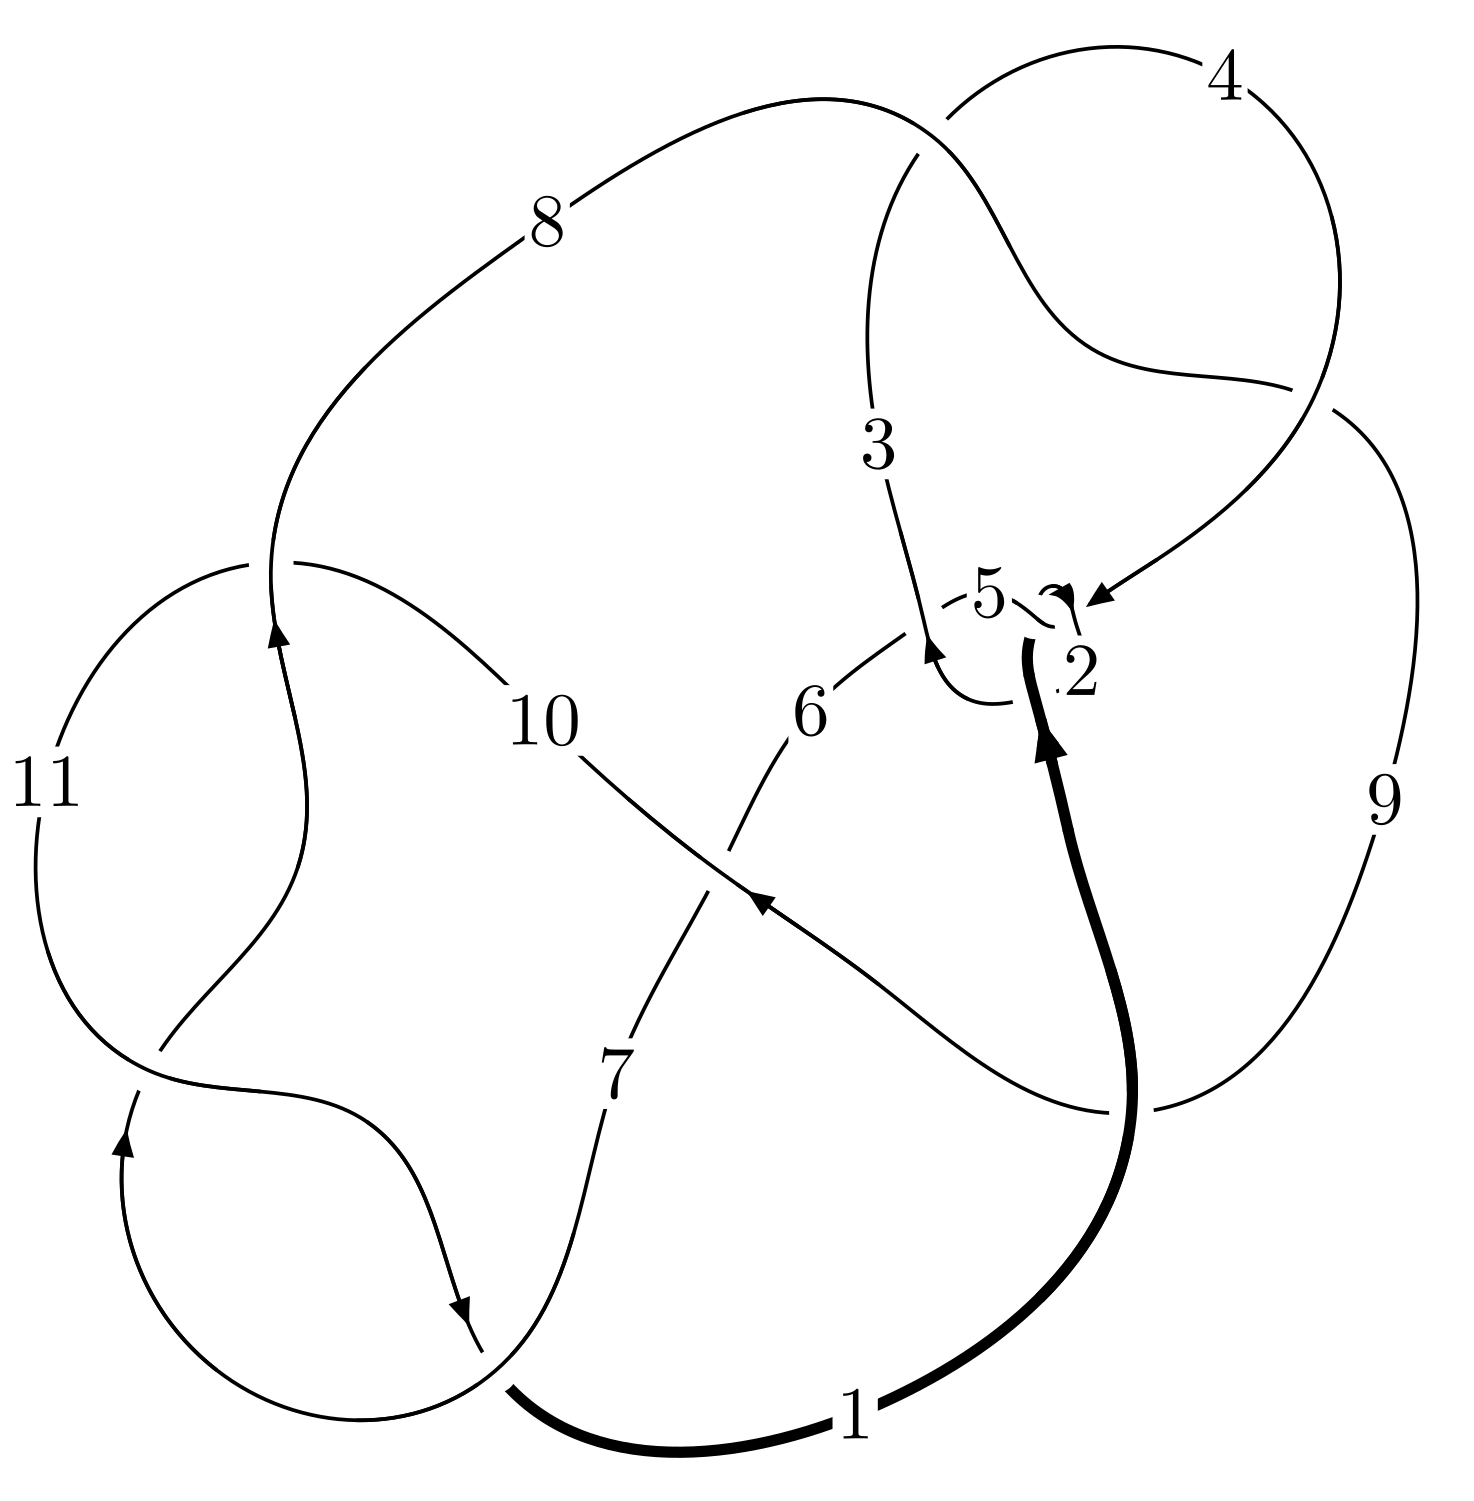
\includegraphics[width=112pt]{../../../GIT/diagram.site/Diagrams/png/632_11n_16.png}\\
\ \ \ A knot diagram\footnotemark}&
\allowdisplaybreaks
\textbf{Linearized knot diagam} \\
\cline{2-2}
 &
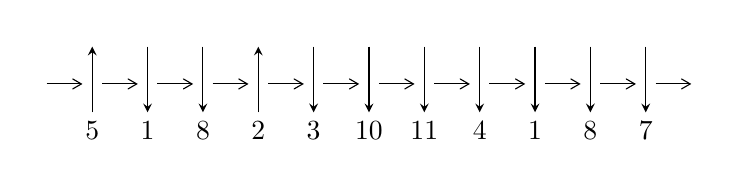
\begin{tikzpicture}[x=20pt, y=17pt]
	% nodes
	\node (C0) at (0, 0) {};
	\node (C1) at (1, 0) {};
	\node (C1U) at (1, +1) {};
	\node (C1D) at (1, -1) {5};

	\node (C2) at (2, 0) {};
	\node (C2U) at (2, +1) {};
	\node (C2D) at (2, -1) {1};

	\node (C3) at (3, 0) {};
	\node (C3U) at (3, +1) {};
	\node (C3D) at (3, -1) {8};

	\node (C4) at (4, 0) {};
	\node (C4U) at (4, +1) {};
	\node (C4D) at (4, -1) {2};

	\node (C5) at (5, 0) {};
	\node (C5U) at (5, +1) {};
	\node (C5D) at (5, -1) {3};

	\node (C6) at (6, 0) {};
	\node (C6U) at (6, +1) {};
	\node (C6D) at (6, -1) {10};

	\node (C7) at (7, 0) {};
	\node (C7U) at (7, +1) {};
	\node (C7D) at (7, -1) {11};

	\node (C8) at (8, 0) {};
	\node (C8U) at (8, +1) {};
	\node (C8D) at (8, -1) {4};

	\node (C9) at (9, 0) {};
	\node (C9U) at (9, +1) {};
	\node (C9D) at (9, -1) {1};

	\node (C10) at (10, 0) {};
	\node (C10U) at (10, +1) {};
	\node (C10D) at (10, -1) {8};

	\node (C11) at (11, 0) {};
	\node (C11U) at (11, +1) {};
	\node (C11D) at (11, -1) {7};
	\node (C12) at (12, 0) {};

	% arrows
	\draw[->,>={angle 60}]
	(C0) edge (C1) (C1) edge (C2) (C2) edge (C3) (C3) edge (C4) (C4) edge (C5) (C5) edge (C6) (C6) edge (C7) (C7) edge (C8) (C8) edge (C9) (C9) edge (C10) (C10) edge (C11) (C11) edge (C12) ;	\draw[->,>=stealth]
	(C1D) edge (C1U) (C2U) edge (C2D) (C3U) edge (C3D) (C4D) edge (C4U) (C5U) edge (C5D) (C6U) edge (C6D) (C7U) edge (C7D) (C8U) edge (C8D) (C9U) edge (C9D) (C10U) edge (C10D) (C11U) edge (C11D) ;
	\end{tikzpicture} \\
\hhline{~~} \\& 
\textbf{Solving Sequence} \\ \cline{2-2} 
 &
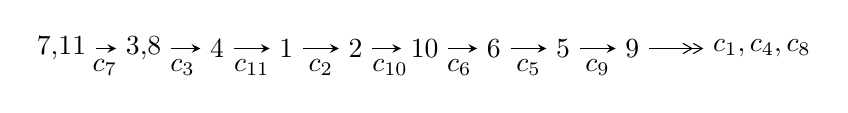
\begin{tikzpicture}[x=25pt, y=7pt]
	% node
	\node (A0) at (-1/8, 0) {7,11};
	\node (A1) at (17/16, 0) {3,8};
	\node (A2) at (17/8, 0) {4};
	\node (A3) at (25/8, 0) {1};
	\node (A4) at (33/8, 0) {2};
	\node (A5) at (41/8, 0) {10};
	\node (A6) at (49/8, 0) {6};
	\node (A7) at (57/8, 0) {5};
	\node (A8) at (65/8, 0) {9};
	\node (C1) at (1/2, -1) {$c_{7}$};
	\node (C2) at (13/8, -1) {$c_{3}$};
	\node (C3) at (21/8, -1) {$c_{11}$};
	\node (C4) at (29/8, -1) {$c_{2}$};
	\node (C5) at (37/8, -1) {$c_{10}$};
	\node (C6) at (45/8, -1) {$c_{6}$};
	\node (C7) at (53/8, -1) {$c_{5}$};
	\node (C8) at (61/8, -1) {$c_{9}$};
	\node (A9) at (10, 0) {$c_{1},c_{4},c_{8}$};

	% edge
	\draw[->,>=stealth]	
	(A0) edge (A1) (A1) edge (A2) (A2) edge (A3) (A3) edge (A4) (A4) edge (A5) (A5) edge (A6) (A6) edge (A7) (A7) edge (A8) ;
	\draw[->>,>={angle 60}]	
	(A8) edge (A9);
\end{tikzpicture} \\ 

\end{tabular} \\

\footnotetext{
The image of knot diagram is generated by the software ``\textbf{Draw programme}" developed by Andrew Bartholomew(\url{http://www.layer8.co.uk/maths/draw/index.htm\#Running-draw}), where we modified some parts for our purpose(\url{https://github.com/CATsTAILs/LinksPainter}).
}\phantom \\ \newline 
\centering \textbf{Ideals for irreducible components\footnotemark of $X_{\text{par}}$} 
 
\begin{align*}
I^u_{1}&=\langle 
2 u^{23}+7 u^{22}+\cdots+2 b-5 u,\;-3 u^{23}-11 u^{22}+\cdots+2 a+8,\;u^{24}+3 u^{23}+\cdots-5 u-1\rangle \\
I^u_{2}&=\langle 
- u^2 a+b,\;u^2 a+a^2+u^2+a- u+2,\;u^3- u^2+2 u-1\rangle \\
\\
\end{align*}
\raggedright * 2 irreducible components of $\dim_{\mathbb{C}}=0$, with total 30 representations.\\
\footnotetext{All coefficients of polynomials are rational numbers. But the coefficients are sometimes approximated in decimal forms when there is not enough margin.}
\newpage
\renewcommand{\arraystretch}{1}
\centering \section*{I. $I^u_{1}= \langle 2 u^{23}+7 u^{22}+\cdots+2 b-5 u,\;-3 u^{23}-11 u^{22}+\cdots+2 a+8,\;u^{24}+3 u^{23}+\cdots-5 u-1 \rangle$}
\flushleft \textbf{(i) Arc colorings}\\
\begin{tabular}{m{7pt} m{180pt} m{7pt} m{180pt} }
\flushright $a_{7}=$&$\begin{pmatrix}1\\0\end{pmatrix}$ \\
\flushright $a_{11}=$&$\begin{pmatrix}0\\u\end{pmatrix}$ \\
\flushright $a_{3}=$&$\begin{pmatrix}\frac{3}{2} u^{23}+\frac{11}{2} u^{22}+\cdots-\frac{33}{2} u-4\\- u^{23}-\frac{7}{2} u^{22}+\cdots+\frac{21}{2} u^2+\frac{5}{2} u\end{pmatrix}$ \\
\flushright $a_{8}=$&$\begin{pmatrix}1\\u^2\end{pmatrix}$ \\
\flushright $a_{4}=$&$\begin{pmatrix}\frac{3}{2} u^{23}+\frac{9}{2} u^{22}+\cdots-\frac{25}{2} u-3\\-\frac{1}{2} u^{22}- u^{21}+\cdots-\frac{5}{2} u-1\end{pmatrix}$ \\
\flushright $a_{1}=$&$\begin{pmatrix}- u\\u\end{pmatrix}$ \\
\flushright $a_{2}=$&$\begin{pmatrix}2 u^{23}+6 u^{22}+\cdots-\frac{27}{2} u-\frac{7}{2}\\-\frac{3}{2} u^{23}-4 u^{22}+\cdots-\frac{1}{2} u-\frac{1}{2}\end{pmatrix}$ \\
\flushright $a_{10}=$&$\begin{pmatrix}u\\u^3+u\end{pmatrix}$ \\
\flushright $a_{6}=$&$\begin{pmatrix}- u^4- u^2+1\\- u^6-2 u^4- u^2\end{pmatrix}$ \\
\flushright $a_{5}=$&$\begin{pmatrix}\frac{1}{2} u^{23}+\frac{3}{2} u^{22}+\cdots-\frac{15}{2} u+1\\-\frac{1}{2} u^{22}- u^{21}+\cdots+\frac{7}{2} u^2-\frac{1}{2} u\end{pmatrix}$ \\
\flushright $a_{9}=$&$\begin{pmatrix}u^5+2 u^3+u\\- u^5- u^3+u\end{pmatrix}$\\ \flushright $a_{9}=$&$\begin{pmatrix}u^5+2 u^3+u\\- u^5- u^3+u\end{pmatrix}$\\&\end{tabular}
\flushleft \textbf{(ii) Obstruction class $= -1$}\\~\\
\flushleft \textbf{(iii) Cusp Shapes $= -2 u^{23}-\frac{9}{2} u^{22}-\frac{45}{2} u^{21}-40 u^{20}-105 u^{19}-\frac{307}{2} u^{18}-\frac{527}{2} u^{17}-325 u^{16}-\frac{757}{2} u^{15}-\frac{803}{2} u^{14}-\frac{589}{2} u^{13}-\frac{531}{2} u^{12}-90 u^{11}-\frac{75}{2} u^{10}+3 u^9+\frac{129}{2} u^8-35 u^7+\frac{15}{2} u^6-\frac{89}{2} u^5-57 u^4-11 u^3-\frac{67}{2} u^2-\frac{3}{2}$}\\~\\
\newpage\renewcommand{\arraystretch}{1}
\flushleft \textbf{(iv) u-Polynomials at the component}\newline \\
\begin{tabular}{m{50pt}|m{274pt}}
Crossings & \hspace{64pt}u-Polynomials at each crossing \\
\hline $$\begin{aligned}c_{1},c_{4}\end{aligned}$$&$\begin{aligned}
&u^{24}+4 u^{23}+\cdots+8 u+1
\end{aligned}$\\
\hline $$\begin{aligned}c_{2}\end{aligned}$$&$\begin{aligned}
&u^{24}+16 u^{23}+\cdots-16 u+1
\end{aligned}$\\
\hline $$\begin{aligned}c_{3},c_{8}\end{aligned}$$&$\begin{aligned}
&u^{24}- u^{23}+\cdots-96 u-64
\end{aligned}$\\
\hline $$\begin{aligned}c_{5}\end{aligned}$$&$\begin{aligned}
&u^{24}-4 u^{23}+\cdots+2 u+1
\end{aligned}$\\
\hline $$\begin{aligned}c_{6}\end{aligned}$$&$\begin{aligned}
&u^{24}+3 u^{23}+\cdots+u-1
\end{aligned}$\\
\hline $$\begin{aligned}c_{7},c_{10},c_{11}\end{aligned}$$&$\begin{aligned}
&u^{24}-3 u^{23}+\cdots+5 u-1
\end{aligned}$\\
\hline $$\begin{aligned}c_{9}\end{aligned}$$&$\begin{aligned}
&u^{24}-13 u^{23}+\cdots-995 u+563
\end{aligned}$\\
\hline
\end{tabular}\\~\\
\newpage\renewcommand{\arraystretch}{1}
\flushleft \textbf{(v) Riley Polynomials at the component}\newline \\
\begin{tabular}{m{50pt}|m{274pt}}
Crossings & \hspace{64pt}Riley Polynomials at each crossing \\
\hline $$\begin{aligned}c_{1},c_{4}\end{aligned}$$&$\begin{aligned}
&y^{24}+16 y^{23}+\cdots-16 y+1
\end{aligned}$\\
\hline $$\begin{aligned}c_{2}\end{aligned}$$&$\begin{aligned}
&y^{24}-12 y^{23}+\cdots-612 y+1
\end{aligned}$\\
\hline $$\begin{aligned}c_{3},c_{8}\end{aligned}$$&$\begin{aligned}
&y^{24}-35 y^{23}+\cdots-13312 y+4096
\end{aligned}$\\
\hline $$\begin{aligned}c_{5}\end{aligned}$$&$\begin{aligned}
&y^{24}-40 y^{23}+\cdots-16 y+1
\end{aligned}$\\
\hline $$\begin{aligned}c_{6}\end{aligned}$$&$\begin{aligned}
&y^{24}-33 y^{23}+\cdots-11 y+1
\end{aligned}$\\
\hline $$\begin{aligned}c_{7},c_{10},c_{11}\end{aligned}$$&$\begin{aligned}
&y^{24}+19 y^{23}+\cdots-11 y+1
\end{aligned}$\\
\hline $$\begin{aligned}c_{9}\end{aligned}$$&$\begin{aligned}
&y^{24}-53 y^{23}+\cdots+17132945 y+316969
\end{aligned}$\\
\hline
\end{tabular}\\~\\
\newpage\flushleft \textbf{(vi) Complex Volumes and Cusp Shapes}
$$\begin{array}{c|c|c}  
\text{Solutions to }I^u_{1}& \I (\text{vol} + \sqrt{-1}CS) & \text{Cusp shape}\\
 \hline 
\begin{aligned}
u &= -0.977245 + 0.071776 I \\
a &= \phantom{-}0.150461 + 0.477664 I \\
b &= -1.86833 + 0.85025 I\end{aligned}
 & -13.8937 + 5.6522 I & -11.88129 - 3.05170 I \\ \hline\begin{aligned}
u &= -0.977245 - 0.071776 I \\
a &= \phantom{-}0.150461 - 0.477664 I \\
b &= -1.86833 - 0.85025 I\end{aligned}
 & -13.8937 - 5.6522 I & -11.88129 + 3.05170 I \\ \hline\begin{aligned}
u &= -0.944342\phantom{ +0.000000I} \\
a &= -0.374599\phantom{ +0.000000I} \\
b &= \phantom{-}1.57977\phantom{ +0.000000I}\end{aligned}
 & -9.62200\phantom{ +0.000000I} & -9.45700\phantom{ +0.000000I} \\ \hline\begin{aligned}
u &= -0.132356 + 1.101640 I \\
a &= \phantom{-}0.224192 - 1.262680 I \\
b &= -1.38202 + 0.85732 I\end{aligned}
 & \phantom{-}2.09684 + 3.39237 I & -6.49952 - 2.22048 I \\ \hline\begin{aligned}
u &= -0.132356 - 1.101640 I \\
a &= \phantom{-}0.224192 + 1.262680 I \\
b &= -1.38202 - 0.85732 I\end{aligned}
 & \phantom{-}2.09684 - 3.39237 I & -6.49952 + 2.22048 I \\ \hline\begin{aligned}
u &= \phantom{-}0.369901 + 1.056050 I \\
a &= \phantom{-}0.19239 - 1.75435 I \\
b &= \phantom{-}0.509437 + 0.688724 I\end{aligned}
 & -1.33599 - 3.11324 I & -9.44737 + 3.66544 I \\ \hline\begin{aligned}
u &= \phantom{-}0.369901 - 1.056050 I \\
a &= \phantom{-}0.19239 + 1.75435 I \\
b &= \phantom{-}0.509437 - 0.688724 I\end{aligned}
 & -1.33599 + 3.11324 I & -9.44737 - 3.66544 I \\ \hline\begin{aligned}
u &= \phantom{-}0.023030 + 1.170740 I \\
a &= \phantom{-}0.00332 + 1.52505 I \\
b &= \phantom{-}0.53462 - 1.45060 I\end{aligned}
 & \phantom{-}3.34786 - 1.42933 I & -3.02808 + 3.24576 I \\ \hline\begin{aligned}
u &= \phantom{-}0.023030 - 1.170740 I \\
a &= \phantom{-}0.00332 - 1.52505 I \\
b &= \phantom{-}0.53462 + 1.45060 I\end{aligned}
 & \phantom{-}3.34786 + 1.42933 I & -3.02808 - 3.24576 I \\ \hline\begin{aligned}
u &= \phantom{-}0.736962 + 0.245534 I \\
a &= \phantom{-}0.482708 + 0.172356 I \\
b &= \phantom{-}1.141730 - 0.517295 I\end{aligned}
 & -3.71809 - 1.00013 I & -12.92204 + 1.61108 I\\
 \hline 
 \end{array}$$\newpage$$\begin{array}{c|c|c}  
\text{Solutions to }I^u_{1}& \I (\text{vol} + \sqrt{-1}CS) & \text{Cusp shape}\\
 \hline 
\begin{aligned}
u &= \phantom{-}0.736962 - 0.245534 I \\
a &= \phantom{-}0.482708 - 0.172356 I \\
b &= \phantom{-}1.141730 + 0.517295 I\end{aligned}
 & -3.71809 + 1.00013 I & -12.92204 - 1.61108 I \\ \hline\begin{aligned}
u &= \phantom{-}0.149866 + 1.301080 I \\
a &= \phantom{-}0.468754 + 1.001100 I \\
b &= -0.632329 - 1.109160 I\end{aligned}
 & \phantom{-}3.26690 - 2.11293 I & -4.50894 + 4.47286 I \\ \hline\begin{aligned}
u &= \phantom{-}0.149866 - 1.301080 I \\
a &= \phantom{-}0.468754 - 1.001100 I \\
b &= -0.632329 + 1.109160 I\end{aligned}
 & \phantom{-}3.26690 + 2.11293 I & -4.50894 - 4.47286 I \\ \hline\begin{aligned}
u &= -0.521270 + 1.255460 I \\
a &= \phantom{-}1.48874 - 0.97432 I \\
b &= -1.105310 - 0.534231 I\end{aligned}
 & -10.25040 - 0.34153 I & -9.34191 - 0.16934 I \\ \hline\begin{aligned}
u &= -0.521270 - 1.255460 I \\
a &= \phantom{-}1.48874 + 0.97432 I \\
b &= -1.105310 + 0.534231 I\end{aligned}
 & -10.25040 + 0.34153 I & -9.34191 + 0.16934 I \\ \hline\begin{aligned}
u &= -0.461477 + 1.300210 I \\
a &= -0.98110 + 1.48411 I \\
b &= \phantom{-}1.37119 - 0.77637 I\end{aligned}
 & -5.57948 + 5.01306 I & -6.18016 - 2.85769 I \\ \hline\begin{aligned}
u &= -0.461477 - 1.300210 I \\
a &= -0.98110 - 1.48411 I \\
b &= \phantom{-}1.37119 + 0.77637 I\end{aligned}
 & -5.57948 - 5.01306 I & -6.18016 + 2.85769 I \\ \hline\begin{aligned}
u &= \phantom{-}0.24692 + 1.39353 I \\
a &= -1.57305 + 0.00181 I \\
b &= \phantom{-}2.02058 - 0.67462 I\end{aligned}
 & \phantom{-}1.55911 - 4.48321 I & -9.00126 + 3.05253 I \\ \hline\begin{aligned}
u &= \phantom{-}0.24692 - 1.39353 I \\
a &= -1.57305 - 0.00181 I \\
b &= \phantom{-}2.02058 + 0.67462 I\end{aligned}
 & \phantom{-}1.55911 + 4.48321 I & -9.00126 - 3.05253 I \\ \hline\begin{aligned}
u &= -0.45937 + 1.35651 I \\
a &= \phantom{-}1.05212 - 2.06998 I \\
b &= -2.35956 + 1.45257 I\end{aligned}
 & -9.4212 + 10.7764 I & -8.42021 - 5.67335 I\\
 \hline 
 \end{array}$$\newpage$$\begin{array}{c|c|c}  
\text{Solutions to }I^u_{1}& \I (\text{vol} + \sqrt{-1}CS) & \text{Cusp shape}\\
 \hline 
\begin{aligned}
u &= -0.45937 - 1.35651 I \\
a &= \phantom{-}1.05212 + 2.06998 I \\
b &= -2.35956 - 1.45257 I\end{aligned}
 & -9.4212 - 10.7764 I & -8.42021 + 5.67335 I \\ \hline\begin{aligned}
u &= \phantom{-}0.450904\phantom{ +0.000000I} \\
a &= \phantom{-}0.305459\phantom{ +0.000000I} \\
b &= -0.393799\phantom{ +0.000000I}\end{aligned}
 & -0.785516\phantom{ +0.000000I} & -12.5270\phantom{ +0.000000I} \\ \hline\begin{aligned}
u &= -0.228245 + 0.158994 I \\
a &= \phantom{-}0.02603 - 2.87156 I \\
b &= -0.322979 - 0.586238 I\end{aligned}
 & -0.34648 - 1.75564 I & -2.27719 + 2.42480 I \\ \hline\begin{aligned}
u &= -0.228245 - 0.158994 I \\
a &= \phantom{-}0.02603 + 2.87156 I \\
b &= -0.322979 + 0.586238 I\end{aligned}
 & -0.34648 + 1.75564 I & -2.27719 - 2.42480 I\\
 \hline 
 \end{array}$$\newpage\newpage\renewcommand{\arraystretch}{1}
\centering \section*{II. $I^u_{2}= \langle - u^2 a+b,\;u^2 a+a^2+u^2+a- u+2,\;u^3- u^2+2 u-1 \rangle$}
\flushleft \textbf{(i) Arc colorings}\\
\begin{tabular}{m{7pt} m{180pt} m{7pt} m{180pt} }
\flushright $a_{7}=$&$\begin{pmatrix}1\\0\end{pmatrix}$ \\
\flushright $a_{11}=$&$\begin{pmatrix}0\\u\end{pmatrix}$ \\
\flushright $a_{3}=$&$\begin{pmatrix}a\\u^2 a\end{pmatrix}$ \\
\flushright $a_{8}=$&$\begin{pmatrix}1\\u^2\end{pmatrix}$ \\
\flushright $a_{4}=$&$\begin{pmatrix}a\\u^2 a\end{pmatrix}$ \\
\flushright $a_{1}=$&$\begin{pmatrix}- u\\u\end{pmatrix}$ \\
\flushright $a_{2}=$&$\begin{pmatrix}- a u+2 a\\u^2 a+a u- a\end{pmatrix}$ \\
\flushright $a_{10}=$&$\begin{pmatrix}u\\u^2- u+1\end{pmatrix}$ \\
\flushright $a_{6}=$&$\begin{pmatrix}u\\- u\end{pmatrix}$ \\
\flushright $a_{5}=$&$\begin{pmatrix}u^2+a+u+1\\u^2 a-2 u+1\end{pmatrix}$ \\
\flushright $a_{9}=$&$\begin{pmatrix}1\\u^2\end{pmatrix}$\\ \flushright $a_{9}=$&$\begin{pmatrix}1\\u^2\end{pmatrix}$\\&\end{tabular}
\flushleft \textbf{(ii) Obstruction class $= 1$}\\~\\
\flushleft \textbf{(iii) Cusp Shapes $= -5 u^2 a+3 a u-5 u^2-4 a+5 u-16$}\\~\\
\newpage\renewcommand{\arraystretch}{1}
\flushleft \textbf{(iv) u-Polynomials at the component}\newline \\
\begin{tabular}{m{50pt}|m{274pt}}
Crossings & \hspace{64pt}u-Polynomials at each crossing \\
\hline $$\begin{aligned}c_{1},c_{2},c_{5}\end{aligned}$$&$\begin{aligned}
&(u^2+u+1)^3
\end{aligned}$\\
\hline $$\begin{aligned}c_{3},c_{8}\end{aligned}$$&$\begin{aligned}
&u^6
\end{aligned}$\\
\hline $$\begin{aligned}c_{4}\end{aligned}$$&$\begin{aligned}
&(u^2- u+1)^3
\end{aligned}$\\
\hline $$\begin{aligned}c_{6},c_{9}\end{aligned}$$&$\begin{aligned}
&(u^3+u^2-1)^2
\end{aligned}$\\
\hline $$\begin{aligned}c_{7}\end{aligned}$$&$\begin{aligned}
&(u^3- u^2+2 u-1)^2
\end{aligned}$\\
\hline $$\begin{aligned}c_{10},c_{11}\end{aligned}$$&$\begin{aligned}
&(u^3+u^2+2 u+1)^2
\end{aligned}$\\
\hline
\end{tabular}\\~\\
\newpage\renewcommand{\arraystretch}{1}
\flushleft \textbf{(v) Riley Polynomials at the component}\newline \\
\begin{tabular}{m{50pt}|m{274pt}}
Crossings & \hspace{64pt}Riley Polynomials at each crossing \\
\hline $$\begin{aligned}c_{1},c_{2},c_{4}\\c_{5}\end{aligned}$$&$\begin{aligned}
&(y^2+y+1)^3
\end{aligned}$\\
\hline $$\begin{aligned}c_{3},c_{8}\end{aligned}$$&$\begin{aligned}
&y^6
\end{aligned}$\\
\hline $$\begin{aligned}c_{6},c_{9}\end{aligned}$$&$\begin{aligned}
&(y^3- y^2+2 y-1)^2
\end{aligned}$\\
\hline $$\begin{aligned}c_{7},c_{10},c_{11}\end{aligned}$$&$\begin{aligned}
&(y^3+3 y^2+2 y-1)^2
\end{aligned}$\\
\hline
\end{tabular}\\~\\
\newpage\flushleft \textbf{(vi) Complex Volumes and Cusp Shapes}
$$\begin{array}{c|c|c}  
\text{Solutions to }I^u_{2}& \I (\text{vol} + \sqrt{-1}CS) & \text{Cusp shape}\\
 \hline 
\begin{aligned}
u &= \phantom{-}0.215080 + 1.307140 I \\
a &= \phantom{-}0.818128 + 0.292480 I \\
b &= -1.52448 - 0.02619 I\end{aligned}
 & \phantom{-}3.02413 - 0.79824 I & -6.43615 - 0.68567 I \\ \hline\begin{aligned}
u &= \phantom{-}0.215080 + 1.307140 I \\
a &= -0.155769 - 0.854759 I \\
b &= \phantom{-}0.73956 + 1.33333 I\end{aligned}
 & \phantom{-}3.02413 - 4.85801 I & -2.88198 + 6.08229 I \\ \hline\begin{aligned}
u &= \phantom{-}0.215080 - 1.307140 I \\
a &= \phantom{-}0.818128 - 0.292480 I \\
b &= -1.52448 + 0.02619 I\end{aligned}
 & \phantom{-}3.02413 + 0.79824 I & -6.43615 + 0.68567 I \\ \hline\begin{aligned}
u &= \phantom{-}0.215080 - 1.307140 I \\
a &= -0.155769 + 0.854759 I \\
b &= \phantom{-}0.73956 - 1.33333 I\end{aligned}
 & \phantom{-}3.02413 + 4.85801 I & -2.88198 - 6.08229 I \\ \hline\begin{aligned}
u &= \phantom{-}0.569840\phantom{ +0.000000I} \\
a &= -0.662359 + 1.147240 I \\
b &= -0.215080 + 0.372529 I\end{aligned}
 & -1.11345 + 2.02988 I & -12.18187 - 4.49037 I \\ \hline\begin{aligned}
u &= \phantom{-}0.569840\phantom{ +0.000000I} \\
a &= -0.662359 - 1.147240 I \\
b &= -0.215080 - 0.372529 I\end{aligned}
 & -1.11345 - 2.02988 I & -12.18187 + 4.49037 I\\
 \hline 
 \end{array}$$\newpage
\newpage\renewcommand{\arraystretch}{1}
\centering \section*{ III. u-Polynomials}
\begin{tabular}{m{50pt}|m{274pt}}
Crossings & \hspace{64pt}u-Polynomials at each crossing \\
\hline $$\begin{aligned}c_{1}\end{aligned}$$&$\begin{aligned}
&((u^2+u+1)^3)(u^{24}+4 u^{23}+\cdots+8 u+1)
\end{aligned}$\\
\hline $$\begin{aligned}c_{2}\end{aligned}$$&$\begin{aligned}
&((u^2+u+1)^3)(u^{24}+16 u^{23}+\cdots-16 u+1)
\end{aligned}$\\
\hline $$\begin{aligned}c_{3},c_{8}\end{aligned}$$&$\begin{aligned}
&u^6(u^{24}- u^{23}+\cdots-96 u-64)
\end{aligned}$\\
\hline $$\begin{aligned}c_{4}\end{aligned}$$&$\begin{aligned}
&((u^2- u+1)^3)(u^{24}+4 u^{23}+\cdots+8 u+1)
\end{aligned}$\\
\hline $$\begin{aligned}c_{5}\end{aligned}$$&$\begin{aligned}
&((u^2+u+1)^3)(u^{24}-4 u^{23}+\cdots+2 u+1)
\end{aligned}$\\
\hline $$\begin{aligned}c_{6}\end{aligned}$$&$\begin{aligned}
&((u^3+u^2-1)^2)(u^{24}+3 u^{23}+\cdots+u-1)
\end{aligned}$\\
\hline $$\begin{aligned}c_{7}\end{aligned}$$&$\begin{aligned}
&((u^3- u^2+2 u-1)^2)(u^{24}-3 u^{23}+\cdots+5 u-1)
\end{aligned}$\\
\hline $$\begin{aligned}c_{9}\end{aligned}$$&$\begin{aligned}
&((u^3+u^2-1)^2)(u^{24}-13 u^{23}+\cdots-995 u+563)
\end{aligned}$\\
\hline $$\begin{aligned}c_{10},c_{11}\end{aligned}$$&$\begin{aligned}
&((u^3+u^2+2 u+1)^2)(u^{24}-3 u^{23}+\cdots+5 u-1)
\end{aligned}$\\
\hline
\end{tabular}\newpage\renewcommand{\arraystretch}{1}
\centering \section*{ IV. Riley Polynomials}
\begin{tabular}{m{50pt}|m{274pt}}
Crossings & \hspace{64pt}Riley Polynomials at each crossing \\
\hline $$\begin{aligned}c_{1},c_{4}\end{aligned}$$&$\begin{aligned}
&((y^2+y+1)^3)(y^{24}+16 y^{23}+\cdots-16 y+1)
\end{aligned}$\\
\hline $$\begin{aligned}c_{2}\end{aligned}$$&$\begin{aligned}
&((y^2+y+1)^3)(y^{24}-12 y^{23}+\cdots-612 y+1)
\end{aligned}$\\
\hline $$\begin{aligned}c_{3},c_{8}\end{aligned}$$&$\begin{aligned}
&y^6(y^{24}-35 y^{23}+\cdots-13312 y+4096)
\end{aligned}$\\
\hline $$\begin{aligned}c_{5}\end{aligned}$$&$\begin{aligned}
&((y^2+y+1)^3)(y^{24}-40 y^{23}+\cdots-16 y+1)
\end{aligned}$\\
\hline $$\begin{aligned}c_{6}\end{aligned}$$&$\begin{aligned}
&((y^3- y^2+2 y-1)^2)(y^{24}-33 y^{23}+\cdots-11 y+1)
\end{aligned}$\\
\hline $$\begin{aligned}c_{7},c_{10},c_{11}\end{aligned}$$&$\begin{aligned}
&((y^3+3 y^2+2 y-1)^2)(y^{24}+19 y^{23}+\cdots-11 y+1)
\end{aligned}$\\
\hline $$\begin{aligned}c_{9}\end{aligned}$$&$\begin{aligned}
&((y^3- y^2+2 y-1)^2)(y^{24}-53 y^{23}+\cdots+1.71329\times10^{7} y+316969)
\end{aligned}$\\
\hline
\end{tabular}
\vskip 2pc
\end{document}